%\documentclass[titlepage]{jsarticle}
%\usepackage{array}
%\usepackage{booktabs}
%\usepackage{amsmath}
%\usepackage[dvipdfmx]{graphicx}
%\usepackage{float}

%\begin{document}

\section{加速器の原理}

本実験では京都大学小型中性子源KUANS(Kyoto University Accelerator-driven Neutron Source)で実験を行った。本節ではこの加速器について説明する。この加速器は中性子を発生させることを目的とした装置である。まず、Proton Linacを用いて、エネルギー$3.5$ MeV、平均電流$100\ \mu$A、ピーク電流$10$ mA、パルス長$30\sim200 \mu$s、繰り返し周波数$20\sim200\ \mu$Hzの陽子ビームを生成する。その後、陽子ビームをBe標的に衝突させ、$^9\rm{Be(p,n)}$反応により中性子を発生させる。このままでは中性子のエネルギーが高すぎて高速中性子となっている。本実験で利用するのはエネルギーの比較的低い熱中性子であるため、Be標的後方の$10\times10\times10$ cm$^3$のポリエチレンブロックにより中性子を減速させる。減速されていない高速中性子は前方に多く含まれているので、ポリエチレンブロックを通過した中性子を陽子ビームに対して90$^{\circ}$の方向で取り出す。

\begin{figure}
\begin{center}
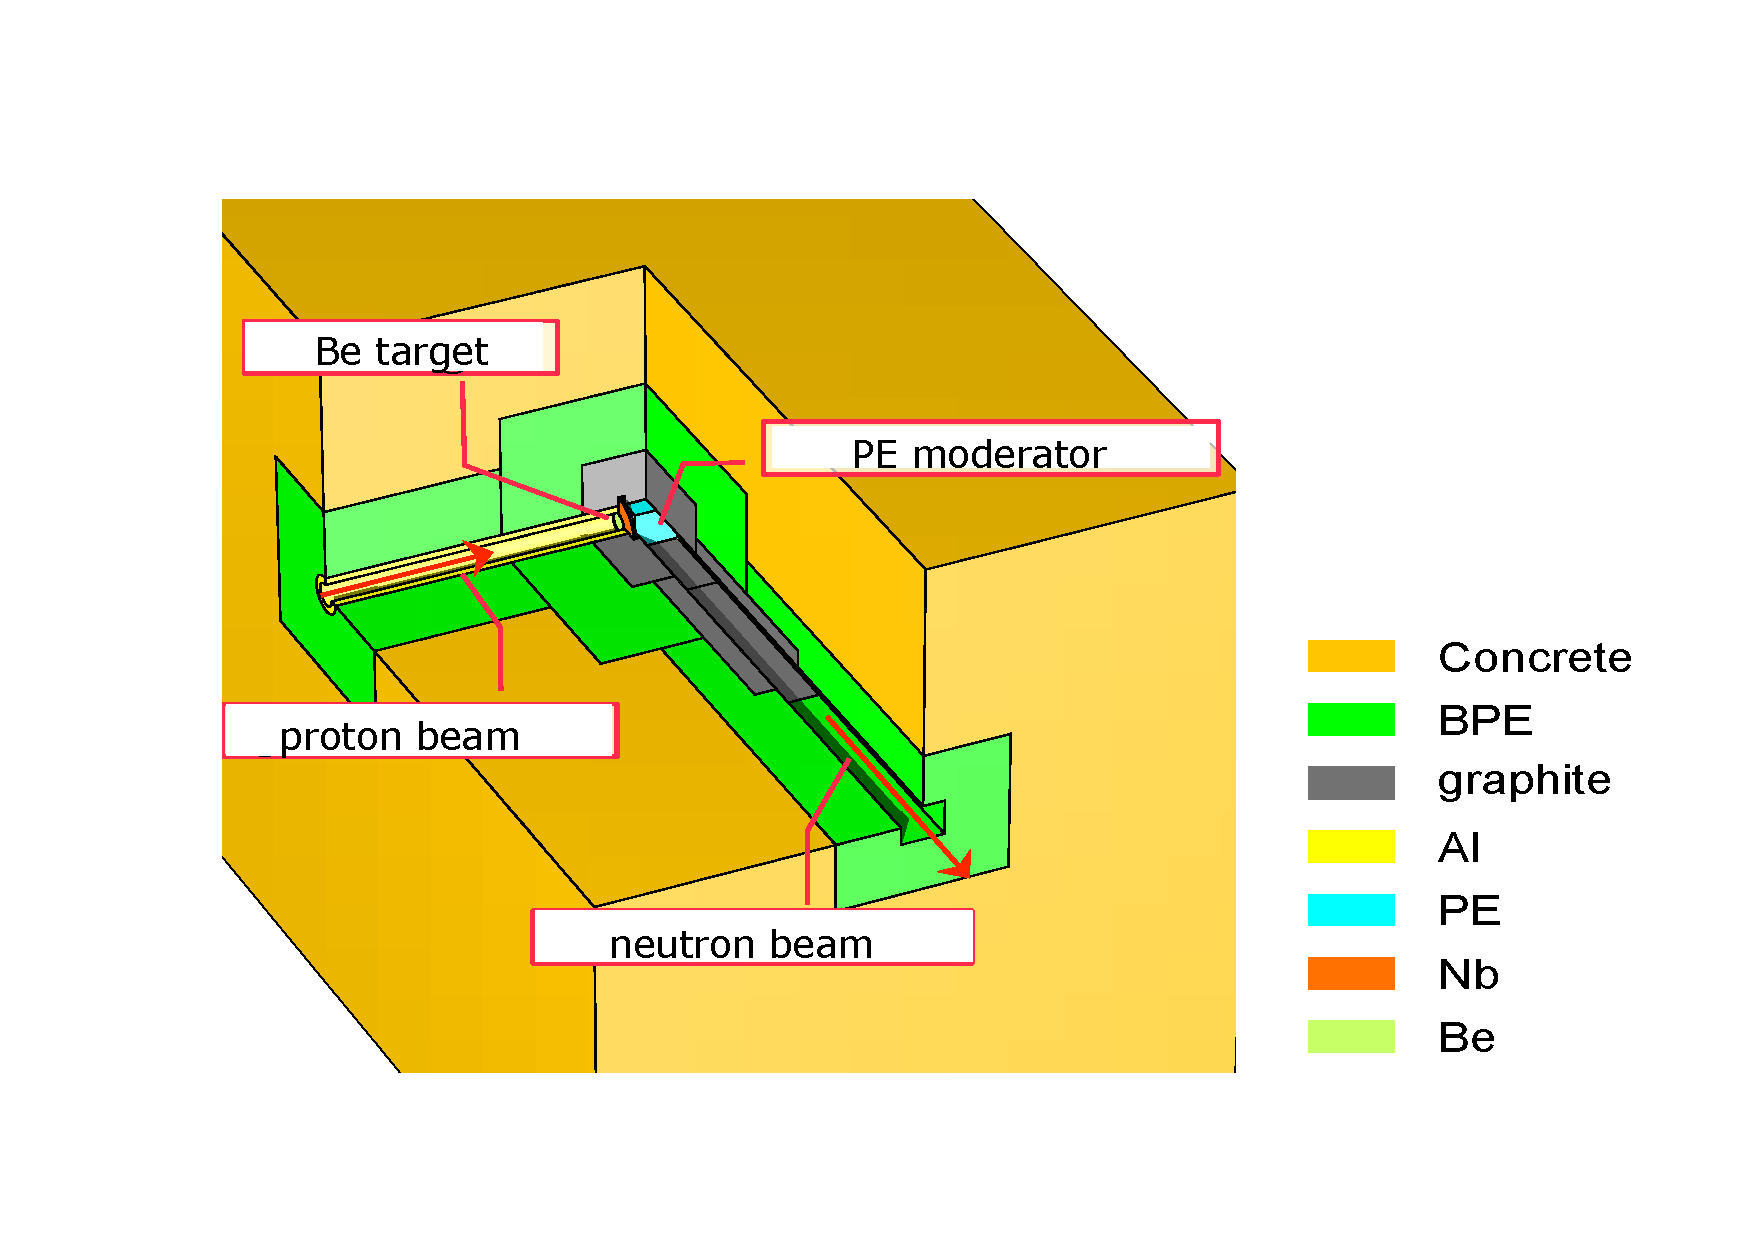
\includegraphics[width=9cm]{accelerator/kuans_inner.pdf}
\caption{KUANSの遮蔽体の内部構造} \label{kuans_inner}
\end{center}
\end{figure}

%\end{document}
